
%(BEGIN_QUESTION)
% Copyright 2010, Tony R. Kuphaldt, released under the Creative Commons Attribution License (v 1.0)
% This means you may do almost anything with this work of mine, so long as you give me proper credit

Suppose three chromatographs are used to measure the composition of feed and separated products in and out of a simple distillation tower:

$$\includegraphics[width=15.5cm]{i02327x01.eps}$$

Based on the chromatogram shown for AT-1, sketch approximate chromatograms for the other two (product) analyzers:

$$\includegraphics[width=15.5cm]{i02327x02.eps}$$

\vfil 

\underbar{file i02327}
\eject
%(END_QUESTION)





%(BEGIN_ANSWER)

This is a graded question -- no answers or hints given!

%(END_ANSWER)





%(BEGIN_NOTES)

Distillation columns separate chemical compounds by boiling point, with lighter (easier-boiling) compounds rising toward the top and heavier (higher-boiling-point) compounds falling toward the bottom.  Chromatographs separate compounds over time by means of those compounds' retention times inside of a packed column.  Generally, lighter molecules travel faster through a column than heavier molecules.  Therefore, the distillate chromatograph should show mostly light molecules (biggest peak being first), while the bottoms chromatograph should show mostly heavy molecules (biggest peak being last):

$$\includegraphics[width=15.5cm]{i02327x03.eps}$$

Note how each of the chromatograms show a little bit of the ``other'' compound in the analysis.  This is because perfect separation is impossible in any distillation column.

%INDEX% Measurement, analytical: chromatography
%INDEX% Process: distillation (generic)

%(END_NOTES)


